% !TeX root = ../../../main.tex
\begin{figure}[htbp]
\begin{ChFiveFloatBody}

\centering
    \begin{minipage}[t]{0.242\textwidth}
    \centering
    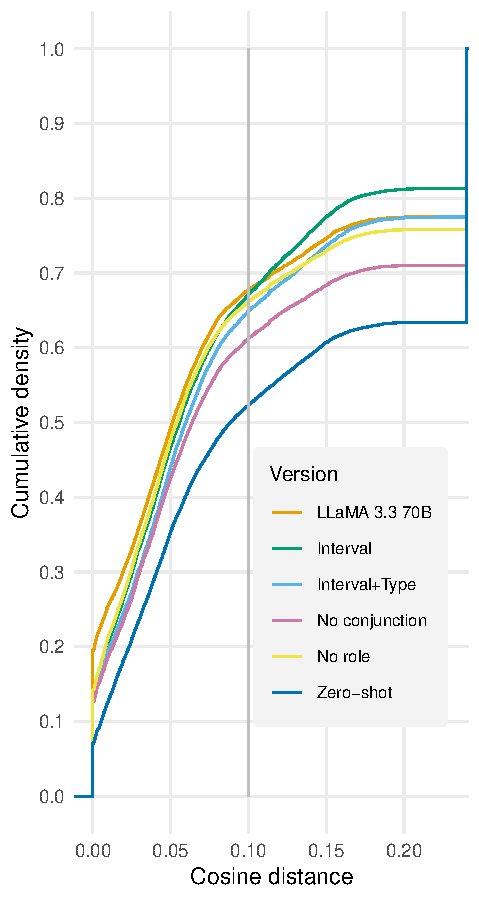
\includegraphics[page=1, width=\linewidth]{Chapters/chapter-05/images/Plots_tables/prompt_ablation_updated_figure.pdf}
    \end{minipage}
    \hfill
    \begin{minipage}[t]{0.242\textwidth}
    \centering
    \includegraphics[page=2, width=\linewidth]{Chapters/chapter-05/images/Plots_tables/prompt_ablation_updated_figure.pdf}
    \end{minipage}
    \hfill
    \begin{minipage}[t]{0.242\textwidth}
    \centering
    \includegraphics[page=3, width=\linewidth]{Chapters/chapter-05/images/Plots_tables/prompt_ablation_updated_figure.pdf}
    \end{minipage}
    \hfill
    \begin{minipage}[t]{0.242\textwidth}
    \centering
    \includegraphics[page=4, width=\linewidth]{Chapters/chapter-05/images/Plots_tables/prompt_ablation_updated_figure.pdf}
    \end{minipage}
    
    
    

\end{ChFiveFloatBody}
\caption{Comparison of \texttt{Llama 3.3 70B} prompt ablation and variant methods for extracting temporal clinical events from case reports. From left to right: (\textbf{A}) event match cumulative distribution function, (\textbf{B}) concordance box plots, (\textbf{C}) time discrepancy from manual annotation timestamps among matched events (overall), and (\textbf{D}) time discrepancy disaggregated by clinician annotator timestamp (time from presentation).}\ChFiveFloatLabel{ch05:fig:prompt_ablation}
\end{figure}